\section{Modified Colonial Competitive Algorithm for the Minimal Hitting Set Problem}
In this paper, we propose a modified colonial competitive algorithm by introducing the concept of independent countries in addition to the existing two types of countries, namely, empires and colonies, in classical CCA.
The three types of countries are defined and explained as follows:
\begin{itemize}
	\item Empire: empires strive to assimilate and possess more colonies in the computational process of the algorithm.
	\item Colony: colonies aim to learn from their corresponding empires in order to grow stronger, with the objective of becoming either independent countries or new empire countries.
	\item Independent country: independent countries try to learn from existing empires and aim to become new empires.
\end{itemize}

With the introduction of independent countries, the MCCA differs from the classical CCA in a number of algorithm stages, including initial country construction, and assimilation and update within empires.
The following sections elaborate these steps in details.


\subsection{Empire initialization}
Given the existence of three types of countries, MCCA uses three parameters to denote the number of each type of country in the initial population, namely, $N_{imp}$, $N_{col}$ and $N_{ind}$, which indicate the number of empires, colonies and independent countries, respectively.
The total number of countries in the initial population is therefore $N_{pop} = N_{imp} + N_{col} + N_{ind}$.
In the initialization step, the algorithm first randomly creates $N_{pop}$ solutions (countries) and selects the best $N_{imp}$ countries as empires, the $N_{col}$ colonies are selected next, and the remaining $N_{ind}$ countries are independent countries. 
The empire construction process in MCCA is the same with that of CCA.
Note that independent countries are not influenced by any empire and therefore not part of any empires.
Figure \ref{fig:fig1} depicts the country classification in the initialization stage.


\begin{figure}[h!]
	\begin{center}
		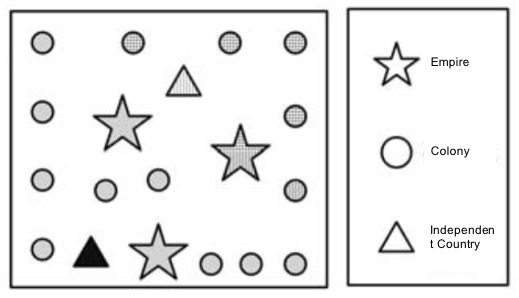
\includegraphics[width=0.5\linewidth]{sections/figure1.jpg}
		\caption{Empire initialization of MCCA}
		\label{fig:fig1}
	\end{center}
\end{figure}


\subsection{Solution encoding}
Solution encoding scheme is the key step in applying CCA to any optimization problems and will greatly affect its performance thereafter.
This paper uses the binary encoding theme, which is one of the most widely used encoding methods due to its simplicity for implementation.

For a set collection $U$, an assimilation step is first conducted to remove all the sets that encompass any other sets, which can greatly reduce the number of hitting sets.
Only the encompassed sets, denoted by $U_i$, are left after the assimilation process. 
Let $n$ indicate the number of sets available in the set collection $U_i$ after the assimilation process.
Let $R$ represent the union of all sets in the set collection, that is, $R = \cup_{i = 1, 2, \cdots, n}U_i, |R| = N$.
It is clear that the minimal hitting set is a proper subset of $R$ and every element in $R$ either exists or does not exist in the minimal hitting set.
Therefore, a binary value can be used to indicate whether an element in $R$ shows up in the minimal hitting set.
In this way, the minimal hitting set can be represented by an array of length $N$ and each element in the array must be a binary value of either 0 or 1.

In order to create good approximations of the minimal hitting set in the initial population, reduce the number of algorithm iterations, and decrease the minimizing calculations, the average number of array elements with value of 1 is set to be close to the number of elements in the minimal hitting set.
Let $X$ denote the average number of elements in the minimal hitting set that have value of 1 and $\beta$ be the probability that an element takes the value of 1, then,
\begin{align}
	\beta = X / N
\end{align}

Since the value of $X$ is unknown in general, the value of $\beta$ must be approximated, which is empirically set to $0.1 \sim 0.5$.
Note that the value of $\beta$ increases when the number of elements in the set, $n$, increases.

Let $Y$ be a chromosome and the gene at the $i$th ($i < N$) position be $x_i$, then $Y = \{x_1, x_2, \cdots, x_N\}$.
The following method is used to create the initial solution based on the binary encoding scheme:
randomly create a number $\xi_i \in (0, 1)$, let $x_i = 1$ if $\xi_i < \beta$; let $x_i = 0$ if $\xi_i \geq \beta$.

\subsection{Fitness function}
The definition of fitness function plays a key role in an algorithm's search efficiency.
The fitness value shows the competitiveness of an solution regarding the objective function and it is also used in the algorithm to decide the solution's capacity to produce offsprings.
Fitness function is often called objective function and is normally used to evaluate individual solution's quality.
The objective function differs for different problems.

In order to assign an objective value to an individual, its closeness to the optimal solution must be evaluated.
For the minimal hitting set problem, there are two necessary conditions: 1) a solution must be a hitting set; 2) any of the solution's proper subset must not be a hitting set.
This paper uses a objective function defined as $f(x) = t$, where $t$ indicates the number of non-empty intersections of the current solution with every set in the set collection.
Note that the number of elements in a set cannot decide whether any proper subset of a set is a hitting set.
The objective function drives a solution to converge to a hitting set, not necessarily a minimal hitting set, and the transformation of the resulting hitting set into a minimal hitting set is required.



\subsection{Minimizing operator}
As discussed in the previous section, the hitting set produced by a solution is not necessarily a minimal hitting set, and the purpose of the minimizing operator in this paper is to convert the resulting superset into a corresponding minimal hitting set.
To this purpose, all individual genes from an solution with value of 1 are converted into 0 and the fitness value is computed.
If the fitness value does not change, the conversion is saved.
This conversion is repeated for each gene within a solution until all genes are converted and the individual will produce a minimal hitting set.

Within an individual, the genes with values of 1 are often related, meaning that whether we can convert a gene from 1 to 0 is affected by other genes with values of 1.
To decide whether elements are related, we need to check the locations corresponding to the elements after assimilation.
If there are two or more elements in the assimilated set, the elements are related; otherwise, they are not related.

If we scan all the genes within a solution chromosome sequentially starting from the first gene, we can find that the probability of converting genes from 1 to 0 is higher for those located in the front of the chromosome than those in the back.
In this case, individuals represented by genes in the front part of the chromosome have higher probability to show up in the minimal hitting set than those located in the back.
In order to assign equal probability to genes regardless of their relative positions on the chromosome, a random scanning scheme is adopted to convert the superset into a minimal hitting set.

The minimizing operator works as follows:
\begin{itemize}
	\item Check whether the current object is  a hitting set or not, if so, go to step (2); otherwise make no changes to the object.
	\item Start scanning the chromosome at position $k$ where $k$ is a random number and $k < N$, convert a gene value from 1 to 0 if applicable and compute its objective value. Keep the change if the resulting solution is a hitting set; otherwise, reverse the change. Let $k = k + 1$. Let the scanning position be $k - N$ if $k \geq N$. After the whole chromosome is scanned, the resulting objective represents a minimal hitting set and copy the distinct components into the final solution.
\end{itemize}


\subsection{Competition}
Similar to the classical CCA, the MCCA needs to calculate the total energy of each empire, which is affected by all the energies of its colonies:
\begin{align}
	E_{C_n} = J_n + \alpha \times \text{mean}\{J_m\}
\end{align}
where $E_{C_n}$ is the total energy of the $n$th empire; $\alpha \in (0, 1)$ is used to control the weight of all the colonies' energies in the final total energy of the empire.
Note that a bigger $\alpha$ value indicates a smaller weight for the empire itself, whereas a smaller $\alpha$ value indicates a bigger weight for the empire.
Normally, $\alpha$ is set to 0.1
In addition, $J_n$ represents all the colonies' energy and $J_m$ is the energy of the $m$th colony of the $n$th empire.

Another similarity between classical CCA and the MCCA is that all the empires try to possess more colonies to increase their total energies.
During the algorithmic process, some empires will have more and more colonies, which will result in some other empires losing their colonies gradually.
The colony competition process works as follows: 1) identify the weakest colony from the empire with the smallest total energy and set the colony as a status of free; 2) all the empires compete for the free colony.
The competition result is decided using a probability value that is associated with the empire's strength, in other words, more powerful empire has higher probability of getting the free colony.

The probability computation requires the normalized total energy of an empire $E_{CN_n}$: 
\begin{align}
	E_{CN_n} = E_{C_n} - \text{max}_{n = 1}^{N_{imp}}\{E_{C_n}\}
\end{align}
where $E_{C_n}$ and $E_{CN_n}$ represent the empire's total energy and normalized total energy, respectively.
The possession probability can therefore be computed as $P_n$:
\begin{align}
	P_n = |E_{CN_n}/\text{max}_{n = 1}^{N_{imp}}\{E_{CN_n}\}|
\end{align}

In order to assign the free colony to an empire, construct the following vector:
\begin{align}
	P = (p_1, p_2, \cdots, p_{N_{imp}})
\end{align}
and another evenly distributed vector $R$ of the same size:
\begin{align}
	R = (r_1, r_2, \cdot, r_{N_{imp}}), \ \ r_1, r_2, \cdots, r_{N_{imp}} \in U(0, 1)
\end{align}
then we get the following vector $D$:
\begin{align}
	D = P-R 
	= (D_1, D_2, \cdots, D_{N_{imp}}) 
	= (p_1 - r_1, p_2 - r_2, \cdots, p_{N_{imp}} - r_{N_{imp}})
\end{align}

Based on the above computations, the free colony will be assigned to the empire with the biggest $D$ value.
The competition process is shown in figure \ref{fig:fig2}.

\begin{figure}[h!]
	\begin{center}
		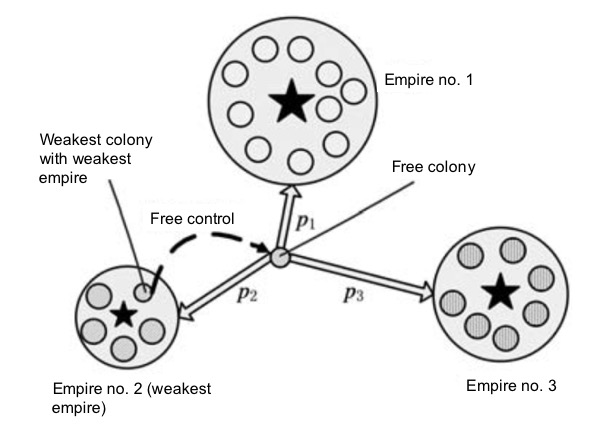
\includegraphics[width=0.5\linewidth]{sections/figure2.jpg}
		\caption{Illustration of colony competition in MCCA}
		\label{fig:fig2}
	\end{center}
\end{figure}

\subsection{Assimilation}
There exist two types of assimilation in the MCCA, namely, assimilation within an empire and assimilation between an empire and an independent country.
The former assimilation process involves only the empire and its colonies and is the same with that of the classical CCA.
The latter assimilation process is described as follows:
\begin{itemize}
	\item An independent country will tentatively move to all empires and the movement process is the same with that of colony to its empire.
	The movement process is achieved by the crossover and mutation operators.
	This paper uses the single-point crossover operator and the mutation operator randomly selects a gene to reverse its current value in order to generate a new solution.
	\item Separate new independent country is generated after the movement toward every empire and the best one is used as the final new independent country.
\end{itemize}

The assimilation processes are depicted in figure \ref{fig:fig3}.
It can be seen from the figure that empire assimilation only involves the empire and its associated colonies, which is different from the assimilation between an independent country and an empire.
The attempts to move to every empire made by an independent country can speed up the algorithm's convergence rate by only selecting the best move; on the other hand, more computational times are required.

\begin{figure}[h!]
	\centering
	\begin{subfigure}[b]{0.4\linewidth}
		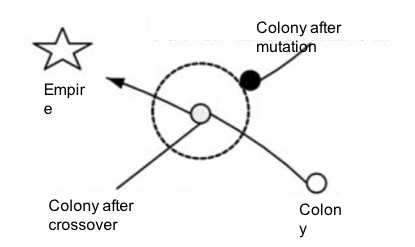
\includegraphics[width=\linewidth]{sections/figure3a.jpg}
		\caption{Assimilation within empire}
	\end{subfigure}
	\begin{subfigure}[b]{0.4\linewidth}
		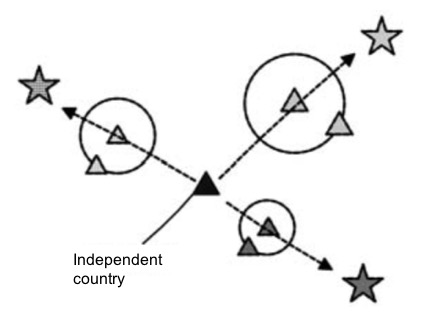
\includegraphics[width=\linewidth]{sections/figure3b.jpg}
		\caption{Assimilation between empire and independent country}
	\end{subfigure}
	\caption{Illustration of assimilation of MCCA}
	\label{fig:fig3}
\end{figure}


\subsection{Update}
There are three types of updating processes in the MCCA, which are depicted in figure \ref{fig:fig4}:
\begin{itemize}
	\item Updating process between an empire and its colonies. If the new colony created after the assimilation process has better objective value than that of the empire, it will become the new empire. The process is illustrated in figure \ref{fig:fig4a}.
	\item Updating process between an independent country and an empire. If the best independent country has better objective value than that of the weakest empire, it will replace the empire and the replaced empire will become an independent country.  The process is depicted in figure \ref{fig:fig4b}.
	\item Updating process between colonies and independent countries. If the best colony after assimilation has better objective value than that of the weakest independent country, it will replace the independent country, which will become a colony. The process is shown in figure \ref{fig:fig4c}.
\end{itemize}

\begin{figure}[h!]
	\centering
	\begin{subfigure}[b]{0.5\linewidth}
		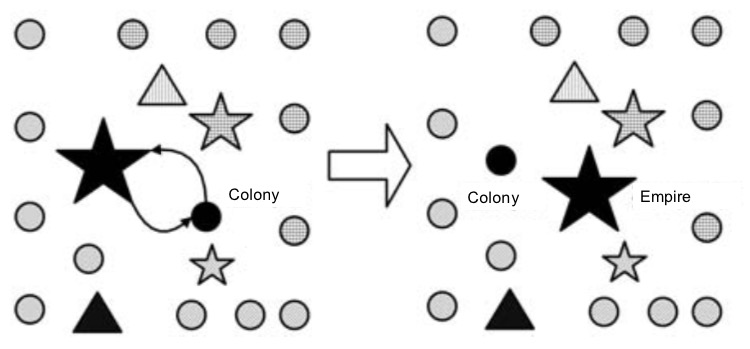
\includegraphics[width=\linewidth]{sections/figure4a.jpg}
		\caption{Update between empire and colony}
		\label{fig:fig4a}
	\end{subfigure}
	\begin{subfigure}[b]{0.5\linewidth}
		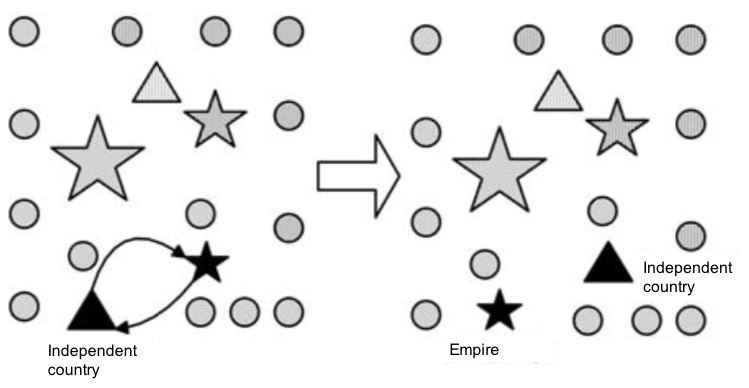
\includegraphics[width=\linewidth]{sections/figure4b.jpg}
		\caption{Update between empire and independent country}
		\label{fig:fig4b}
	\end{subfigure}
	\begin{subfigure}[b]{0.5\linewidth}
		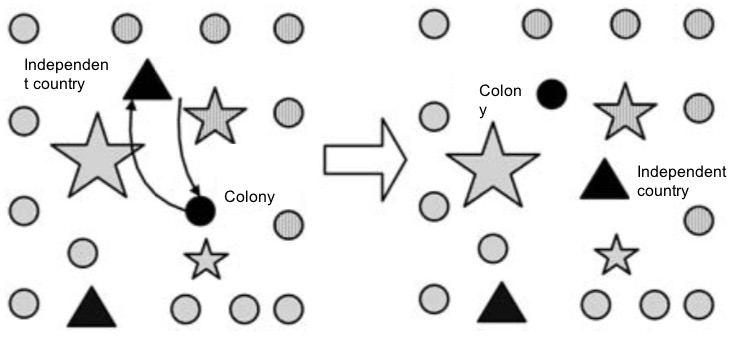
\includegraphics[width=\linewidth]{sections/figure4c.jpg}
		\caption{Update between colony and independent country}
		\label{fig:fig4c}
	\end{subfigure}
	\caption{Illustration of updating processes in MCCA}
	\label{fig:fig4}
\end{figure}

\subsection{Empire removal}
The MCCA uses the same empire removal step as in the classical CCA.